\documentclass{article}
\usepackage{mathtools}
\usepackage{stmaryrd}
\usepackage{amsmath,amssymb}
\usepackage{graphicx}
\usepackage{xspace}
\usepackage{mypackage}
\usepackage{amsthm}
\usepackage{hyperref}

\newtheorem{theorem}{Theorem}[section]
\newtheorem{lemma}[theorem]{Lemma}
\newtheorem{corollary}[theorem]{Corollary}
\theoremstyle{definition}
\newtheorem{definition}[theorem]{Definition}
\newtheorem{example}[theorem]{Example}
\newtheorem{claim}[theorem]{Claim}
\newtheorem*{claim*}{Claim}
\theoremstyle{remark}


\title{Small Complexity Classes for Operators}
\author{Akitoshi Kawamura \and Hiroyuki Ota}
\date{\today}


\begin{document}
\maketitle
\begin{abstract}
Computable Analysis is a branch of computability theory that
studies real numbers or real functions computable on digital machines.
We use the framework of Type-two Theory of Effectivity proposed by Weihrauch,
which is based on the models by Turing, Grzegorczyk and Lacombe.
Not only computability, but also time and space complexity of real functions, 
has been studied since Ko's work in the 1980s. 
In this field,
we analyze the complexity of algorithms in numerical analysis 
and discuss lower bounds on the speed of reliable numerical algorithms.


Kawamura and Cook proposed an extended framework for TTE.
They define type-two complexity classes analogous to $\classP$, $\classNP$,
and $\classPSPACE$ by bounding time or space by the second-order polynomial
in the size of the input.
In this thesis, we focus on small classes
and define type-two analogues of the log-space class $\classL$ and
the circuit class $\classNC$.
We also define the type-two $\classP$-completeness under suitable log-space reductions.

We apply this framework to some specific problems.
First, we study the complexity of the problem to find the roots of
the polynomial from its coefficients.
Using Mosier's analysis, we can bound the required input precision 
by a polynomial in the precision of the solution.
We combine this analysis and the discrete result 
that the problem to approximate the roots of the polynomial with integer 
coefficients is $\classNC$ computable,
and we show that the polynomial roots are type-two $\classNC$ computable.
Second, we give two examples of $\classP$-complete operators,
the inverse operation and the fix-point operation on contracting mappings.
It is known that these operators are $\classP$-complete in a non-uniform sense:
the fix-points of $\classNC$-computable contracting mappings,
as well as the inverse function $f^{-1}$ of a one-to-one $\classL$-computable function $f$,
can be $\classP$-complete.
We express these theorems in the uniform way and
show that these operators themselves are type-two $\classP$-complete.
\end{abstract}

\section{Introduction}

\subsection{Computable analysis}

We investigate the computational complexity of several problems in 
numerical analysis.
The problems we study in this thesis are of the following kind:
How much resource is needed to compute the roots of a polynomial?
Which operators on real function are feasibly computable but inherently sequential?
In this paper, we use the model of the real computation from the field of 
Computational Analysis.

\emph{Computable Analysis} 
\cite{ko1991complexity,weihrauch00:_comput_analy}
studies real functions that are computable approximately 
by digital (finite-precision floating-point) machines.
Here, polynomial-time computability and other notions of complexity 
is from this field and measure how hard it is to approximate real functions
with specified precision  (Sect.~\ref{section:TTE}). 

In the theory of \emph{real computation}, 
there is no ``Church-Turing thesis''.
Church-Turing thesis states that a function on finite strings or natural 
numbers is ``effectively'' or algorithmically computable 
if and only if some Turing machine can compute it.
Many other computation models such as $\lambda$-calculus or recursion
were proposed and shown to be equivalent to Turing machine.
In contrast, there are models about computation on real numbers, 
and some of them are known not to be equivalent to others.
Another model is the Blum-Shub-Smale (BSS) machine \cite{blum1988theory}.
The main difference between BSS machines and machines in Computable Analysis is
that a BSS machine has registers containing real numbers with infinite precision
while digital machine can work on finite-precision number.
Because of this difference,
machines in Computable Analysis cannot compute noncontinuous functions
but the algorithm described in Computable Analysis 
can be used as numerical computation in real computers
 while we do not know
how to realize BSS machines.

\subsection{Type-two complexity theory for small classes}
The complexity of an operation $F$ on real functions
is stated indirectly in the non-uniform form like
\begin{quote}
 if $f$ is in the complexity class $\classonefont X$,
 then $F(f)$ is in the complexity class $\classonefont Y$, and \\
 there is $f$ in $\classonefont X$ such that $F(f)$ is hard for
 the complexity class $\classonefont Z$.
\end{quote}
That is, there is some restriction to apply the framework TTE
to complexity theory.
There is a widely-recognized definition of polynomial-time computable 
real functions whose domain is compact.
However, there is not such a model for
operators $F$ on real functions in purpose to state
directly that $F$ is polynomial-time computable or hard for $\classPSPACE$.

Kawamura proposed an extension of this framework \cite{kawamura2012complexity}.
The key idea is representing uncountable 
objects by \emph{length-monotone} string functions, which make it possible to define the
\emph{size} of function and to bound resources by size of input.
In that framework we can state directly about the complexity of
 an operator $F$ in the effective or uniform form like
\begin{quote}
 $F$ is in the complexity class $\mathcal Y$, and \\
 $F$ is hard for $\mathcal Z$ under the $\mathcal X$ reduction,
\end{quote}
where $\mathcal{X, Y, Z}$ are type-two complexity classes analogous to $\classonefont{X, Y, Z}$.
There is no obvious way to define consistent type-two classes 
analogous to usual (type-one) complexity classes.

First, we introduce new small type-two classes.
Type-two analogues of the classes $\classP$, $\classNP$, and $\classPSPACE$
are defined by bounding resource of oracle machines by using 
second-order polynomials on the size of the input string functions,
\cite{kawamura2012complexity}.
Using second-order logarithmic function,
we define type-two classes analogous to the logarithmic-space 
complexity class $\classL$ and the circuit complexity class $\classNC$, 
which are both contained in $\classP$.
While there are various models of relativized logarithmic space,
we choose the \emph{constant stack machine} \cite{aehlig2007relativizing} 
since it is consistent with relativized circuit complexity classes 
and it makes some elemental operation log-space computable.
We also define $\classP$-completeness under log-space reductions.

Informally speaking, operators in type-two $\classL$ have
memory friendly algorithm and operators in type-two $\classNC$
are parallelizable.
If an operation is $\classP$-complete,
it is feasibly computable but inherently sequential. 

Then, we apply this framework to several problems in analysis.
Our first application is the problem of finding roots of a polynomial 
from its coefficients.
In numerical analysis, it is known to be generally ill-conditioned, 
that is, the roots are sensitive to 
small errors in the coefficients \cite{wilkinson1963rounding}.
However, with the complex analysis by Mosier \cite{mosier1986root},
we can bound the precision needed to compute
roots by a polynomial in the required precision of the solution.
We combine this analysis with the discrete result 
that the problem to approximate the roots of the polynomial with integer 
coefficients is $\classNC$ computable \cite{neff1994specified}
to show that roots of a polynomial with real coefficients
is $\classNC$ computable.
Second application is about $\classP$-complete operators.
There exist a few result about $\classP$-completeness of problems of numerical analysis:
The inverse function $f^{-1}$ can be $\classP$-complete under the log-space
reduction even if $f$ is log-space computable \cite{ko1983computational};
The fix-points of contracting mappings can be $\classP$-complete under the
$\classNC$ reduction even if contracting mappings are all $\classNC$ computable \cite{hoover1991real}.
We express these theorems in constructive way and
show type-two $\classP$-completeness of these operators.




%Chap.~\ref{chapter:computable-analysis} introduces Type-two Theory of Effectivity, the framework of Computable Analysis.
%We review basic concepts of TTE in Sect.~\ref{section:TTE} and
%Kawamura's extended framework for TTE in Sect.~\ref{section:TTF}.
%In Sect.~\ref{section:small-classes}, we introduce our new type-two classes
%$\classLtwo$ and $\classNCtwo$.
%We also define $\classPtwo$-completeness under reductions using these small classes.
%In Chap.~\ref{chapter:applications}, we investigate the complexity of some analytic problems.
%In Sect.~\ref{section:function}, we prove that finding roots of a polynomial 
%from coefficients is $\classNC$ computable.
%In Sect.~\ref{section:P-complete}, we show the $\classP$-completeness of 
%the inverse operation and the fix-point operation.
%In Sect.~\ref{section:differentiable}, we study the complexity of
%smooth differential equations.
%Most part in that section only depends on Sect.~\ref{section:TTE}
%since we mainly discuss in non-uniform way.
%We summarize this thesis and discuss about future works in Chap.~\ref{chapter:conclusion}.


\paragraph{Notation}
Let $\N$, $\Z$, $\Q$, $\R$ denote the set of natural numbers,
integers,
rational numbers and 
real numbers, respectively.

We assume that any polynomial is increasing,
since it does not change the meaning of 
polynomial-time computable or polynomial-space computable.

A {\em multi-value function} (or {\em multi-function}) $F$ from $X$ to $Y$,
denoted $F \colon X \rightrightarrows Y$,
is a subset of $X \times Y$.
For $x \in X$, we write $F[x]$ for the set of $y \in Y$ such that $(x,y) \in F$.
The domain of $F$, denoted by $\dom F$, is the set of $x \in X$ such that 
$F[x]$ is not empty.
If $F[x]$ has only one element of $Y$, we write $F(x)$ for the unique element.
We say $F$ is a {\em partial function} if $F[x]$ has a unique element for all
$x \in \dom F$.
We say $F$ is a {\em total function} or simply a {\em function} 
if $F[x]$ has a unique element for all $x \in X$.

\section{Framework of Computable Analysis}
\label{section: computable analysis}
In the first three subsections,
we review the framework TTE
to define new type-two classes corresponding to small complexity classes.
We define basic concepts of TTE in Sect.~\ref{section:TTE},
such as polynomial-time computable functions and hardness of real function
for the (usual type-one) complexity class $\classP$ \cite{ko1991complexity}.
In Sect.~\ref{section:TTF}, we extend TTE using second-order polynomials
in the size of input functions \cite{kawamura2012complexity}.
Our new type-two classes $\classLtwo$ and $\classNCtwo$ are defined in Sect.~\ref{section:small-classes}.
We also define $\classPtwo$-completeness under suitable reductions using these small classes.

\subsection{Type-two Theory of Effectivity}
\label{section:TTE}

This section reviews the complexity notions 
in Computable Analysis~%
\cite{ko1991complexity,weihrauch00:_comput_analy}. 
We start by fixing an encoding of real numbers 
by string functions.

\begin{definition}
 A function $\phi \colon \{0, 1\} ^* \to \{0, 1\} ^*$ is a \emph{name} of a real number $x$ 
 if for all $n \in \N$,
  $\phi(0^n)$ is the binary representation of $\lfloor x \cdot 2^n \rfloor$ or
  $\lceil x \cdot 2^n \rceil$,
 where $\lfloor \cdot \rfloor$ and $\lceil \cdot \rceil$ mean
 rounding down and up to the nearest integer.
\end{definition}

In effect, a name of a real number $x$ receives $0 ^n$ and 
returns an approximation of $x$ with precision $2 ^{-n}$.

We use \emph{oracle Turing machines} (henceforth just \emph{machines})
to work on these names (Fig.~\ref{fig:model-of-function}).
Let $M$ be a machine and $\phi$ be a function from strings to strings. 
We write $M ^\phi (0 ^n)$ for the output string 
when $M$ is given
$\phi$ as oracle and string $0^n$ as input.
Thus, we also regard $M^\phi$ as a function from strings to strings.

\begin{figure}
 \begin{center}
  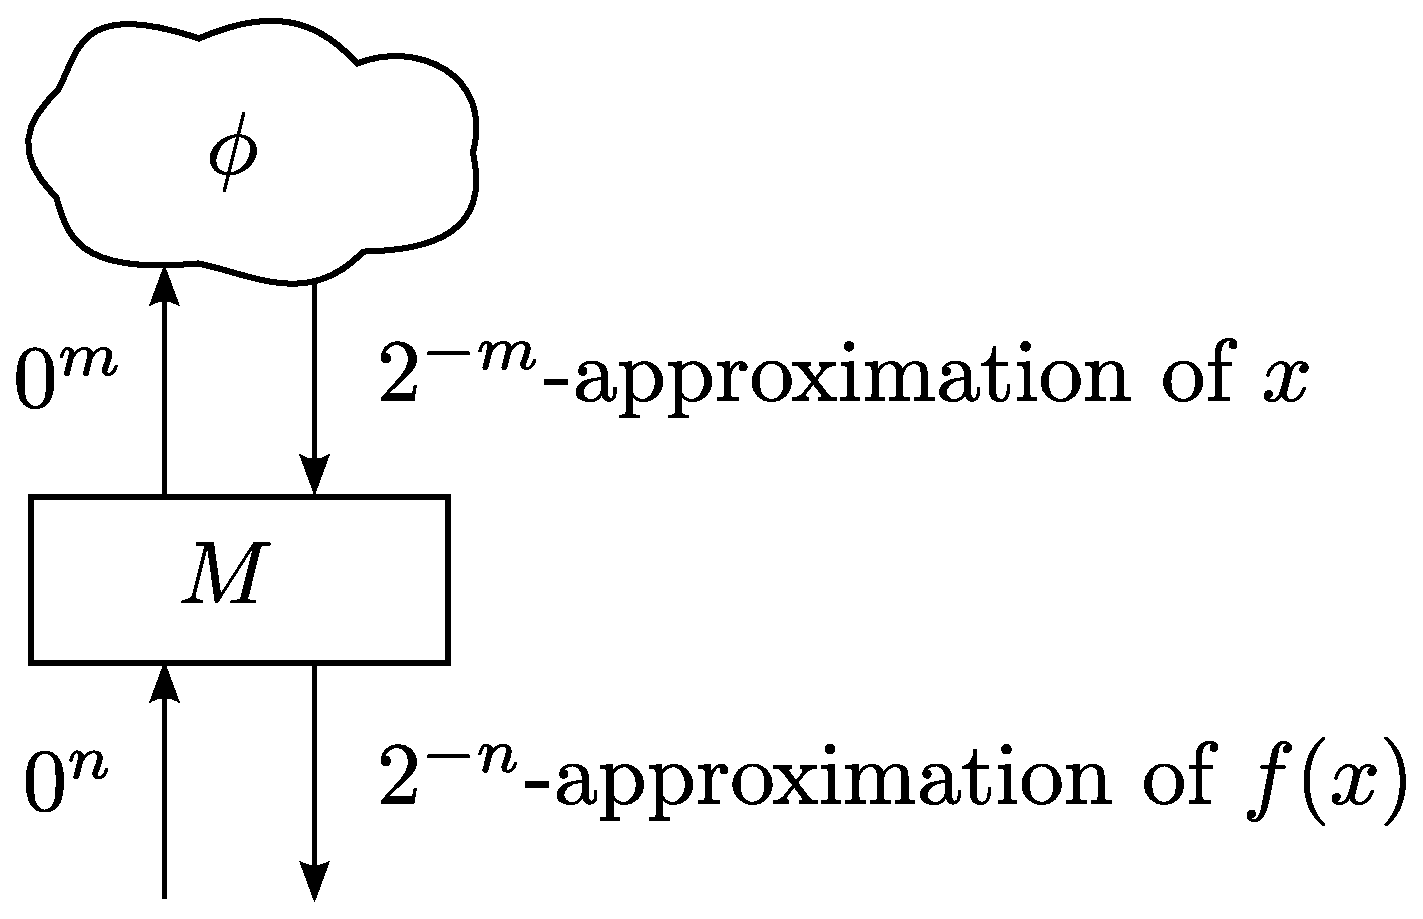
\includegraphics[height=0.17\textheight]{image/model-of-function.eps}
 \end{center}
 \caption{A machine $M$ computing a real function $f$}
 \label{fig:model-of-function}
%% \phi _xを\phiにする
\end{figure}

\begin{definition}
Let $A$ be a bounded closed interval of\/ $\R$.
A machine $M$ \emph{computes} a real function $f \colon A \to \R$ 
if for any $x \in A$ and any name $\phi$ of it,
$M ^\phi$ is a name of $f(x)$.
\end{definition}

Computation of a function $f \colon A \to \R$ on
a two-dimensional bounded closed region $A \subseteq \R ^2$ 
is defined in a similar way using machines with two oracles.
A real function is (\emph{polynomial-time}) \emph{computable} if there exists some machine that computes it (in polynomial time).
Polynomial-time computability of a real function $f$ means that
for any $n \in \N$, 
an approximation of $f(x)$ with error bound $2^{-n}$
is computable in time polynomial in $n$ 
independent of the real number $x$.

By the time the machine outputs the approximation of $f (x)$ of precision~$2 ^{-n}$, 
it knows $x$ only with some precision $2 ^{-m}$.
This implies that all computable real functions are continuous.
If the machine runs in polynomial time,
this $m$ is bounded polynomially in $n$.
This implies \eqref{eq:modulus} in the following lemma, 
which characterizes polynomial-time real functions
by the usual polynomial-time computability of string functions 
without using oracle machines. 

\begin{lemma}
 \label{lem:type1representation}
 A real function is polynomial-time computable if and only if
 there exist a polynomial-time computable function 
 $\phi \colon (\Q \cap [0, 1]) \times \{0\} ^* \to \Q$ and 
 polynomial $p \colon \N \to \N$ such that
 for all $d \in \Q \cap [0,1]$ and $n \in \N$,
 \begin{equation}
  |\phi(d, 0^n) - f(d)| \le 2^{-n},
 \end{equation}
 and for all $x, y \in [0, 1]$, $n \in \N$,
 \begin{equation} 
  |x-y| \le 2^{-p(n)} \Rightarrow |f(x) - f(y)| \le 2^{-n},
   \label{eq:modulus}
 \end{equation}
where each rational number is written
as a fraction whose numerator and denominator
are integers in binary.
\end{lemma}

To talk about hardness, we define reduction. 
A language $L \subseteq \{0, 1\} ^*$ is identified with the function
$L \colon \{0, 1\} ^* \to \{0, 1\}$ such that $L (u) = 1$ when $u \in L$.

\begin{definition} \label{definition: reduction}
 A language $L$ \emph{reduces} to a function $f \colon [0, 1] \to \R$
 if there exists a polynomial-time function $S$ and a polynomial-time oracle Turing machine $M$ (Fig.~\ref{fig:reduction})
 such that for any string $u$, 
  \begin{enumerate}
   \item $S(u, \cdot)$ is a name of a real number $x_u$, and 
   \item $M^\phi(u)$ accepts if and only if $u \in L$ for any name $\phi$ of $f(x_u)$.
  \end{enumerate}
\end{definition}
This reduction may look stronger (and hence the reducibility weaker) than
the one in Kawamura~\cite{kawamura2010lipschitz} 
in that $M$ can make multiple queries adaptively, 
but this makes no difference, 
because the lengths of these queries 
are bounded by a polynomial in $\lvert u \rvert$, 
and the longest query gets all the information that any shorter query gets. 

For a complexity class~$C$, a function $f$ is \emph{$C$-hard}
if all languages in $C$ reduce to $f$.

 \begin{figure}
  \begin{center}
  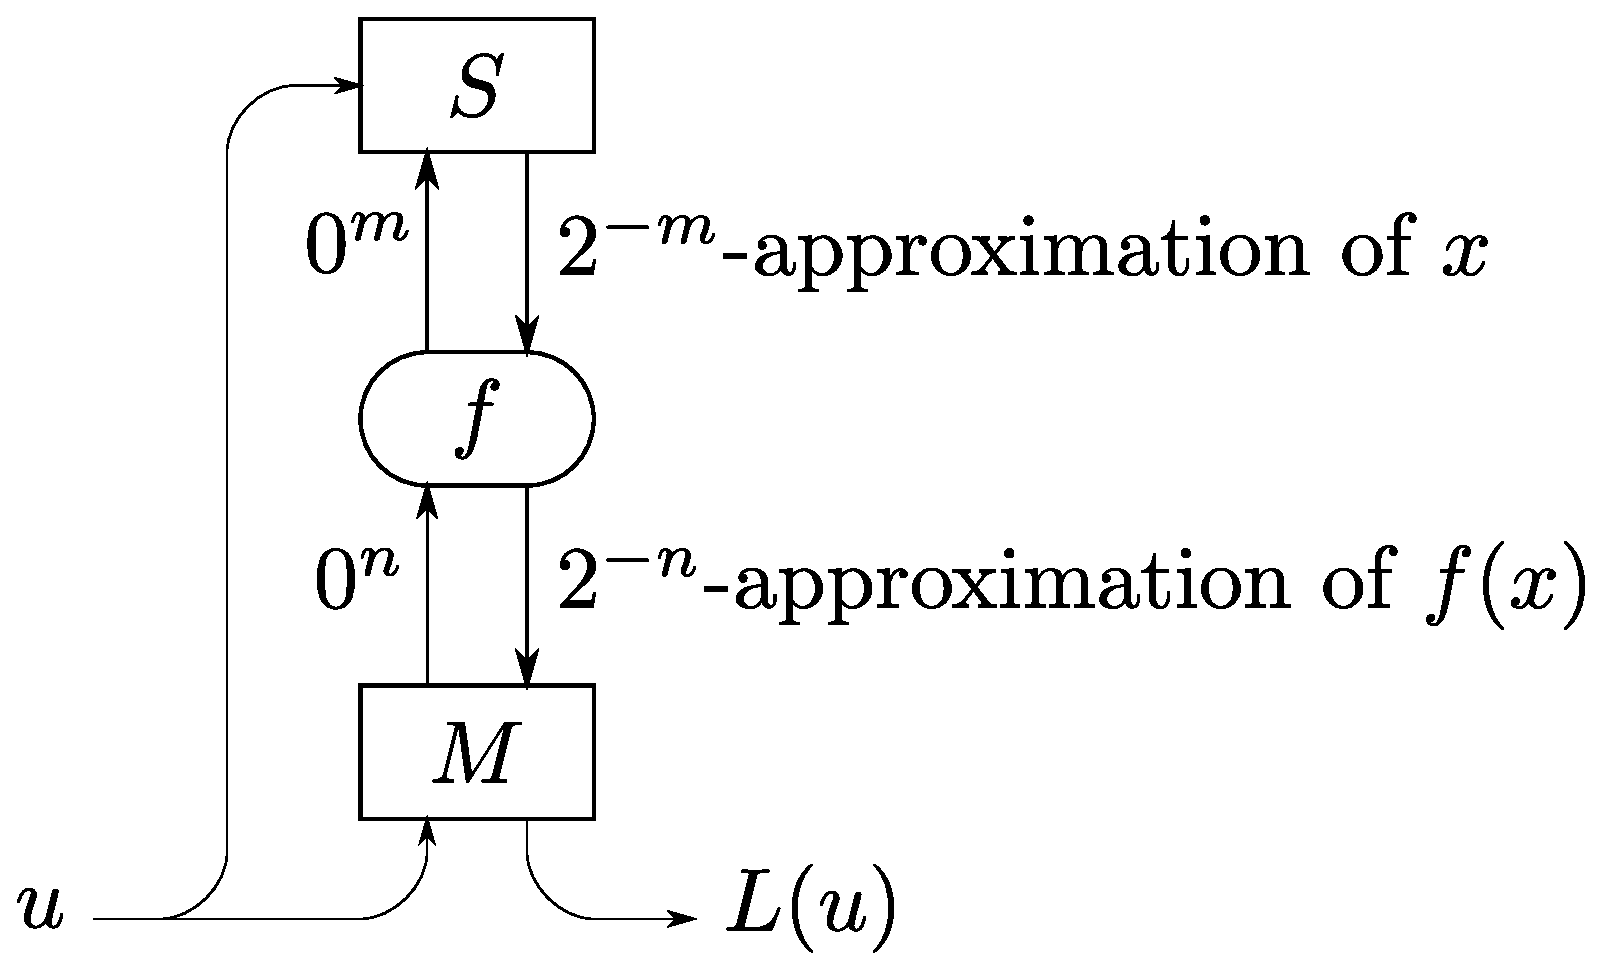
\includegraphics[scale=0.25]{image/reduction.eps}
  \caption{Reduction from a language $L$ to a function $f \colon [0,1] \to \R$}
  \label{fig:reduction}
  \end{center}
 \end{figure}

\subsection{Second-order polynomial}
\label{section:TTF}

This section reviews the extended framework of Computable Analysis~%
\cite{kawamura2012complexity}.
A (total) function $\phi \colon \Sigma^* \to \Sigma^*$ is \emph{length monotone}
if  $|\phi(u)| \le |\phi(v)|$ whenever $|u| \le |v|$.
The set of length monotone functions is denoted $\LM$.
We write $\Pred$ for the set of functions $\phi \colon \Sigma^* \to \{0, 1\}$.
Since $|\phi(u)| = |\phi(v)| = 1$ for all $\phi \in \Pred$ and $u, v \in \Sigma^*$,
$\Pred$ is a subset of $\LM$.

\begin{definition}
 A machine $M$ computes a multi-function $A \colon \LM \rightrightarrows \LM$ if for any
 $\phi \in \dom A$, there is $\psi \in A[\phi]$ such that $M^\phi(u) = \psi(u)$ for all $u \in \Sigma^*$.
\end{definition}

The \emph{size} of a length monotone $\phi$, denoted $|\phi|$,
is a (non-decreasing) function from $\N$ to $\N$ defined by 
$|\phi|(|u|) = |\phi(u)|$.
This is well-defined since a length monotone function maps 
strings of the same length to strings of the same length.

\emph{Second-order polynomials} in type-1 variable $L \colon \N \to \N$
and type-0 variable $n \in \N$ 
are defined inductively as follows:
a positive integer is a second-order polynomial;
the variable $n$ is a second-order polynomial;
$P+Q$, $P \cdot Q$ and $L(P)$ are
second-order polynomials if $P$ and $Q$ are second-order polynomials.
Note that if $P$ is a second-order polynomial and $L$ is a (usual) first-order
polynomial, then $P(L)$ is a first-order polynomial.

\begin{definition}
\begin{enumerate}
 \item We write $\classFPtwo$ (resp. $\classFPSPACEtwo$) for the class of
       multi-functions from $\LM$ to $\LM$ computed by a machine that runs
       in second-order polynomial time (resp. space).
 \item We write $\classPtwo$ (resp. $\classPSPACEtwo$) for the class of
       multi-functions from $\LM$ to $\Pred$ computed by a machine that runs
       in second-order polynomial time (resp. space).
\end{enumerate}
\end{definition}

\begin{lemma}
 \begin{enumerate}
  \item Functions in $\classFPtwo$ (resp. $\classFPSPACEtwo$) map 
	length-monotone functions in $\classFP$ to $\classFP$ 
	(resp. $\classFPSPACE$).
  \item Functions in $\classPtwo$ (resp. $\classPSPACEtwo$) map 
	length-monotone functions in $\classFP$ to $\classP$
	(resp. $\classPSPACE$).
 \end{enumerate}
\end{lemma}





For the (basic) representations of real numbers and real functions,
we use $\rhoR$ and $\deltabox$ \cite{kawamura2012complexity}.
For each $n \in \N$, let $\D_n$ denote the set of strings of the form
\begin{equation}
 sx/1\!\underbrace{00\dots0}_{n},
\end{equation}
where $s$ is the sign and $x \in \{0,1\}^*$.
We write $D$ for the union $\cup_n \D_n$.
We regard $D$ as the set of fractions of binary numbers
and write $\llbracket u \rrbracket$ for the number encoded by $u \in \D$.

We call $\phi \in \LM$ as a $\rhoR$-name of $x \in \R$ 
if $\phi(0^i) \in \D$ and $\llbracket \phi(0^i) - x \rrbracket \le 2^{-i}$
for all $i \in \N$.

Let $\phi \colon \{0\}^* \times \D \to \D$ be length-monotone and $\mu \colon \N \to \N$ be non-decreasing,
$\langle \overline{\mu}, \phi \rangle$ is a {\em $\deltabox$-name} of $f \in \classC[0,1]$
if and only if $\mu$ is a modulus of continuity of $f$
and $|\llbracket \phi(0^n, d) \rrbracket - f(d)| \le 2^{-n}$ for all $n \in \N$ and $d \in \D|_{[0,1]}$.




\subsection{New type-two classes for small complexity}
\label{section:small-classes}

In this section, we introduce new type-two complexity classes
corresponding to log-space $\classL$ and circuit complexity $\classNC$
based on the framework we reviewed in the previous section.
We also define $\classP$-completeness under log-space reductions.

\subsubsection{Logarithmic space}
There are several versions of relativized log-space computation
\cite{aehlig2007relativizing,buss1988relativized,ladner1976relativization,wilson1988measure, ota2013logspace}.
Here, we define type-two log-space computation 
by extending \emph{stack model with constant height} by Aehlig, Cook and Nguyen 
\cite{aehlig2007relativizing},
since it is consistent with relativized circuit complexity classes 
and it makes some elemental operation log-space computable.
See the comment of Theorem~\ref{theorem:inclusion}.
In their paper language oracles,
 length monotone function as oracle.
Hence, we add read-only tape that oracle writes answers to stack machines.
The answer tape is magically erased when a machine \emph{pushes},
that is it starts writing a new query tape.

\begin{definition}
 A (constant-stack) machine $M$ runs in (second-order) \emph{logarithmic space}
 if there is a second-order polynomial $P$ such that for all $\phi \in \LM$
 and $u \in \Sigma^*$, $M^\phi(u)$ visits at most $\log(P(|\phi|)(|u|))$ cells
 in work tape.
\end{definition}

\begin{definition}
 We write $\classFLtwo$ as a set of multi-functions from $\LM$ to $\LM$
 computed by a constant-stack machine that runs in second-order logarithmic space.
 We write $\classLtwo$ as a set of multi-functions from $\LM$ to $\Pred$
 computed by a constant-stack machine that runs in second-order logarithmic space.
\end{definition}

\begin{lemma}
\label{lemma:Ltwo-maps-L-to-L}
\mbox{}
\begin{enumerate}
 \item Functions in $\classFLtwo$ map length-monotone functions in $\classFL$
       to length-monotone functions in $\classFL$.
 \item Functions in $\classLtwo$ map length-monotone functions in $\classFL$
       to languages $\classL$.
\end{enumerate}
\end{lemma}

\begin{proof}
We only show (1) and (2) is provable in analogous argument.
For all $\phi \in \classFL$, $\log(P(|\phi|)(|u|)) = O(\log(|u|))$
since there is a polynomial $p$ such that $|\phi|(n) \le p(n)$.
$\classFL$ is closed under relativization, that is $\classFL^\classFL = \classFL$.
So functions computed by constant-stack machines with $\classFL$ oracle are in $\classFL$.
\end{proof}


\subsubsection{Circuit complexity classes}
\paragraph{Oracle circuits}


Let $n, m \in \N$ and $L \colon \N \to \N$ be a non-decreasing function.
An \emph{$n$-input $m$-output circuit relative to size-$L$ oracle} is a circuit with
$n$ inputs and $m$ outputs consisting of 
$\NOT$ $(\neg)$, $\OR$ $(\vee)$, $\AND$ $(\wedge)$, oracle $(\phi)$ gates,
where each $\NOT$ gate has only one input and each $\phi$ gate with $k$ inputs
has $L(k)$ outputs.
The size of $C$, denoted by $|C|$, is the number of gates.
The depth of $C$, denoted by $\depth(C)$, is the length of the longest path
from inputs to outputs.
Let $x \in \{0, 1\}^*$ be an input, $\phi \in \LM$ be an oracle and
$C$ be a $|x|$-input $|\phi|$-oracle $m$-output circuit,
we write the output of $C$ as $C^\phi(x)$.
More formally, we define as below.

\begin{definition}[Oracle circuits]
Let $n, m \in \N$ and $L \colon \N \to \N$ be a non-decreasing function.
A \emph{$n$-input $m$-output circuit relative to size-$L$ oracle} is 
a labeled directed acyclic graph with $n$ sources and $m$ sinks.
All vertexes except sources are labeled with $\{\NOT, \OR, \AND\}$
or $\{\phi_i\}_{i \in \N}$.
In-degree of $\NOT$ vertexes is $1$ and
$\phi_i$ vertex with $k$ in-degree satisfies $L(k) > i$.


The size of $C$, denoted by $|C|$, is the number of vertexes.
The depth of $C$, denoted by $\depth(C)$, is the length of the longest path in $C$.
Let $x \in \{0, 1\}^*$ be an input, $\phi \in \LM$ be an oracle and
$C$ be $|x|$-input $m$-output circuit relative to size-$|\phi|$ oracle.
The output of $C$ is denoted by $C^\phi(x) \in \{0, 1\}^m$,
where each logic gate performs the logical operation on its inputs
and $\phi_i(x) = 1$ if and only if the $i$th bit of $\phi(x)$ is 1.
\end{definition}



\paragraph{\texorpdfstring{$\classAC^i$ and $\classNC$}{ACi and NCi}}

A circuit family $(C_{L,n})_{L,n}$ is a set of circuit
such that $C_{L, n}$ is an $n$-input circuit relative to size-$L$ oracle
for all $n \in \N$ and non-decreasing function $L \colon \N \to \N$.

\begin{definition}
 We say \emph{a circuit family $(C_{L,n})_{L,n}$ computes multi-function 
 $A \colon \LM \to \LM$} if for all $\phi \in \dom A$, 
 there is $\psi \in A[\phi]$ satisfying $\psi(x) = C_{|\phi|, |x|}^\phi(x)$
 for all $x \in \Sigma^*$.
\end{definition}

A circuit family $(C_{L,n})_{L,n}$ is \emph{(second-order) polynomial size}
if there is a second-order polynomial $P$ satisfying
$|C_{L,n}| \le P(L)(n)$ for all $n \in \N$ and non-decreasing functions
$L \colon \N \to \N$.

\begin{definition}
 Let $k$ be an integer.
 We write $\classFACtwo^k$ (resp. $\classACtwo^k$) for the class of 
 multi-function from $\LM$ to $\LM$ (resp. to $\Pred$) computed by
 a polynomial-size circuit family $(C_{L,n})_{L,n}$ such that
 there is a second-order polynomial $P$ satisfying
 $\depth(C_{L,n}) \le \log^k(P(L)(n))$ for all $n \in \N$ and non-decreasing
 $L \colon \N \to \N$.
 We write $\classFNCtwo$ and $\classNCtwo$ for the hierarchies
 $\cup_{i \in \N} \classFACtwo^i$ and $\cup_{i \in \N} \classACtwo^i$.
\end{definition}


\begin{lemma}
\label{lemma:NCtwo-maps-NC-to-NC}
\mbox{}
\begin{enumerate}
 \item Functions in $\classFACtwo^i$ map length-monotone functions in $\classFAC^j$ into $\classFAC^{i+j}$.
 \item Functions in $\classACtwo^i$ map length-monotone functions in $\classFAC^j$ into $\classAC^{i+j}$.
\end{enumerate}
\end{lemma}

\begin{proof}
We only show (1).
Since for all $\phi in \classFAC^j \cap \LM$, there is a polynomial $p$ satisfying $|\phi|(n) \le p(n)$, 
$(C^\phi_{|\phi|,n})_n$ is (first-order) polynomial size and its depth is $O(\log^i(n))$.
Let $(D_n)_n$ is a circuit family computing $\phi$ whose depth is $O(\log^j(n))$.
The circuit family given by replacing oracle gates in $(C^\phi_n)_n$ by $(D_n)_n$ is polynomial size and its depth is $O(\log^{i+j}(n))$.
\end{proof}

\begin{corollary}
\mbox{}
\begin{enumerate}
 \item Functions in $\classFNCtwo$ map length-monotone functions in $\classFNC$ into $\classFNC$.
 \item Functions in $\classNCtwo$ map length-monotone functions in $\classFNC$ into $\classNC$.
\end{enumerate} 
\end{corollary}



\paragraph{Uniformity}


For each non-decreasing function $L \colon \N \to \N$, 
we write $0^L$ for the length-monotone function mapping 
$u \in \Sigma^*$ to $0^{L(|u|)}$.

\begin{definition}[$\Luniform$ circuit families]
A circuit family $(C_{L,n})_{L,n}$ is \emph{$\classLtwo$ uniform} if there is a function $A \in \classFLtwo$ computing the description of $C_{L,n}$ on input $0^n$ with oracle $0^L$ for all $n \in \N$ and non-decreasing $L \colon \N \to \N$.
\end{definition}

\begin{theorem}
[$\classFPtwo = \Luniform\ \classFPtwo\!\text{/poly}$]
\label{theorem:P-equals-L-uniform-P-poly}
A multi-function $A$ from $\LM$ to $\LM$ is computed by a polynomial-size
$\Luniform$ circuit family if and only if $A \in \classFPtwo$.
\end{theorem}

\begin{proof}
 It is obvious that machines can compute the output of
 polynomial-size $\Luniform$ circuits in polynomial time.
 The if part is provable in the similar argument to the proof of
 $\classP \subseteq \classL\uniform\ \classP\!\text{/poly}$.
 For each multi-function $A \in \classFPtwo$, there is an oracle machine $M$
 computing $A$ whose head movements do not depend on the input $x$ or oracle
 $\phi$ but only depend on the input length $|x|$ and oracle size $|\phi|$.
 This property enable a polynomial-size $\Luniform$ circuit family to simulate $M$.
\end{proof}

Type-two classes keep the inclusion relation of type-one classes
since we choose stack machine as the log-space oracle machine.

\begin{theorem}
\label{theorem:inclusion}
\begin{equation}
 \Luniform\ \classACtwo^0
 \subseteq \classLtwo 
 \subseteq \Luniform\ \classNCtwo
 \subseteq \classPtwo
\end{equation}
\end{theorem}

\begin{proof}
 The first inclusion can be proved in a similar way
 to show $\classL\uniform\ \classAC^0 \subseteq \classL$.
 The second inclusion follows from that fact 
 $\classLtwo \subseteq \Luniform\ \classACtwo^1$ 
 that can be proved in a similar argument to 
 the proof of $\text{cs}\classL(\alpha) \subseteq \classAC^1(\alpha)$
 \cite{aehlig2007relativizing}.
 The third inclusion immediately follows from
$
 \Luniform\ \classNCtwo \subseteq \Luniform\ \classPtwo\text{\!/poly} = \classPtwo.
$
\end{proof}


The following lemma suggests that type-two $\classLtwo$ uniformity respects
$\classL$ uniformity.
\begin{lemma}
 Let $(C_{L,n})_{L,n}$ be a (second-order) polynomial-size $\Luniform$ oracle circuit family
 and $(D_n)_n$ be a (first-order) polynomial-size $\classL$-uniform circuit family.
 A circuit family given by replacing oracle gates in $(C_{L,n})_{L,n}$ with
 $(D_n)_n$ is $\classL$ uniform.
\end{lemma}

\begin{proof}
 Let $A \colon \LM \to \LM$ be a function computing the description of $(C_{L,n})_{L,n}$,
 $B \colon \Sigma^* \to \Sigma^*$ be a function computing the description of $(D_n)_n$, and
 $L \colon \N \to \N$ be the size of oracle $(D_n)_n$, i.e.
 the function mapping $n$ to the output length of $D_n$.
 The function $A(0^L)$ is in $\classFL$ since $0^L \in \classFL$ and $A \in \classFLtwo$.
 Since given $A(0^L)$ and $B$ as oracles,
 computing the description of the circuit family given by replacing oracle
 gates in $(C_{L,n})_{L,n}$ with $(D_n)_n$ is log-space computable
 and $\classFL$ is closed under relativization,
 it is log-space computable.
\end{proof}

\begin{corollary}
\mbox{}
\begin{enumerate}
 \item Functions in $\Luniform\ \classFACtwo^i$ 
       map length-monotone functions in $\classL$-uniform $\classFAC^j$ 
       to $\classL\text{-uniform }\classFAC^{i+j}$.
 \item Functions in $\Luniform\ \classACtwo^i$ 
       map length-monotone functions in $\classL$-uniform $\classFAC^j$ 
       to $\classL\text{-uniform }\classAC^{i+j}$.
 \item Functions in $\Luniform\ \classFNC$
       map length-monotone functions in $\classL$-uniform $\classFNC$ 
       to $\classL\text{-uniform }\classFNC$.
 \item Functions in $\Luniform\ \classNC$
       map length-monotone functions in $\classL$-uniform $\classFNC$ 
       to $\classL\text{-uniform }\classNC$.
\end{enumerate}
\end{corollary}




\subsubsection{Reductions and completeness}
\paragraph{Reductions}
We define the paring function, denoted by $\langle \phi, \psi \rangle$,
of length-monotone functions as follows:%
\footnote{
The pairing function is defined as
$\langle \phi, \psi \rangle(0u) = \phi(u) 0^{|\psi(u)|}$
and 
$\langle \phi, \psi \rangle(1u) = \psi(u) 1^{|\phi(u)|}$ 
in \cite{kawamura2010complexity}.
In this definition, however, we cannot distinguish $\phi(u)$ and the padding
if $\phi$ is a length-monotone function from $\Sigma^*$ to $\{0\}^*$,
so we put $1$ to separate the padding.
}
$\langle \phi, \psi \rangle(0u) = \phi(u) 10^{|\psi(u)|}$ and 
$\langle \phi, \psi \rangle(1u) = \psi(u) 10^{|\phi(u)|}$.
We pad $0$s to make the pairing function length-monotone.
We write $\langle \phi, \psi, \theta \rangle$ 
for $\langle \phi, \langle \psi, \theta \rangle \rangle$, and so on.


\begin{definition}
Let $A$ and $B$ be multi-functions from $\LM$ to $\LM$.
\begin{itemize}
 \item $A$ is \emph{many-one log-space reducible} to $B$, 
       denoted $A \redLmF B$,
       if there are functions $r, s, t \in \classFLtwo$ such that 
       for all $\phi \in \dom A$,
       $s(\phi) \in \dom B$ and each $\theta \in B[s(\phi)]$ satisfies that
       the function maps $x \in \Sigma^*$ to $r(\phi)(x, \theta(t(\phi)(x)))$
       is in $A[\phi]$.
 \item $A$ is \emph{Weihrauch log-space reducible} to $B$,
       denoted $A \redLmF B$,
       if there are functions $r, s \in \classFLtwo$ such that 
       for all $\phi \in \dom A$,
       $s(\phi) \in \dom B$ and each $\theta \in B[s(\phi)]$ satisfies that
       $r(\langle \phi, \theta \rangle)$ is in $A[\phi]$.
\end{itemize}
Let $A$ and $B$ be multi-functions from $\LM$ to $\Pred$.
\begin{itemize}
 \item $A$ is \emph{many-one log-space reducible} to $B$, denoted 
       $A \redLm B$, if there are functions $s, t \in \classFLtwo$ such that 
       for all $\phi \in \dom A$, $s(\phi) \in \dom B$ and each 
       $\theta \in B[s(\phi)]$ satisfies that $\theta \circ t(\phi)$ is in $A[\phi]$.
\end{itemize} 
\end{definition}

These reductions are log-space analogous to the polynomial-time reductions 
$\redmF^2$, $\redW^2$, $\redm^2$ \cite{kawamura2012complexity}.
We define the $\classNC$ reductions $\redmF^\classNCtwo$, $\redW^\classNCtwo$,
and $\redm^\classNCtwo$ by replacing $\classFLtwo$ with $\classNCtwo$.
Many-one reduction $\redmF$ is a special case of Weihrauch reduction $\redW$,
so if $A \redmF B$ then $A \redW B$.

There is another version of a many-one reduction defined by
Beame et al. \cite{beame1995relative}.
We define log-space analogous to it as follows:
We write $A \redLB B$ if there are function $r, s, t \in \classFLtwo$
if there are functions $r, s, t \in \classFLtwo$ such that 
for all $\phi \in \dom A$,
$s(\phi)(x, \cdot) \in \dom B$ and each $\theta \in B[s(\phi)(x, \cdot)]$ 
satisfies that the function maps $x \in \Sigma^*$ 
to $r(\phi)(x, \theta(t(\phi)(x)))$ is in $A[\phi]$.
This reduction is much stronger than others since
it can use the input string $x$ while making the input of $B$.
The reduction $\redLmF$ is a special case of $\redLB$ where
$s$ does not depend on the string input $x$.
See the comments after the next lemma and before Lemma~\ref{lemma:P-hard-g_u} for
the disadvantage and the advantage of this reduction.

Let $\classtwofont{C}$ be a set of multi-functions from $\LM$ to $\LM$.
A multi-function $B$ from $\LM$ to $\LM$ is \emph{$\classtwofont{C}$-$\leq$-hard} if $A \leq B$ for all $A \in \classtwofont{C}$,
and $B$ is \emph{$\classtwofont{C}$-$\leq$-complete} 
if $B$ is $\classtwofont{C}$-$\leq$-hard and in $\classtwofont{C}$.

Let $F$ be a subset of $\LM$.
We write $\cup F$ for a multi-function mapping $x \in \Sigma^*$ to 
$\{f(x) \mid f \in F\}$.

\begin{lemma}
\label{lemma:P-complete}
Let $B$ be a $\classFPtwo$-$\redLmF$-complete multi-function.
There is $\psi \in \dom B \cap \classFL$ satisfying that
 $\cup (B[\psi])$ is $\classFP$-$\le^\classL_{\mathrm{mF}}$-complete.
\end{lemma}

We will use this lemma to reduce constructive results
($\classFPtwo$-$\redLmF$-hardness of an operation) to a non-constructive 
results (the existent of $\classFP$-hard solution).
This lemma would not have been true, if in the definition 
of reductions like $\redLB$ \cite[Lemma~3.6]{kawamura2012complexity}.
That is a disadvantage of the reduction of Beame et al.

\begin{proof}
Let $A \colon \LM \to \LM$ be the constant function mapping each $\phi \in \LM$ to \emph{Circuit Value Problem} ($\probCVP$), which is $\classFP$-$\redmF$-complete function.
Since $\probCVP \in \classFP$, $A \in \classFPtwo$.
Let $r, s, t \in \classFLtwo$ be functions which reduces $A$ to $B$
as the definition of $\redLmF$.
Choose any $\phi \in \classFL$, and it follows from Lemma~\ref{lemma:Ltwo-maps-L-to-L}
that $r(\phi), s(\phi), t(\phi) \in \classFL$.
Let $\psi = s(\phi)$, then $r(\phi)$ and $s(\phi)$ give the reduction that
$A(\phi) \redmF^\classL \cup (B[\psi])$.
Since $\probCVP$, equal to $A(\phi)$, is $\classFP$-$\redmF^\classL$-complete,
so is $\cup (B[\psi])$.
\end{proof}


\paragraph{P-complete problems}

We define a partial function $\probDTIMEtwo$ from $\LM$ to $\Pred$ as follows:
The domain $\dom \probDTIMEtwo$ is a set of $\langle M, \overline \mu, \phi \rangle$
such that $M$ is a (program of) machine, $\mu \colon \N \to \N$ is non-decreasing, $\phi \in \LM$, and $M^\phi(x)$ stops in $\mu(|x|)$ steps for all $x \in \Sigma^*$.
$\probDTIMEtwo(\langle M, \overline \mu, \phi \rangle)(x)$ is $1$ if
$M^\phi(x)$ accepts, otherwise it is 0.

\begin{lemma}
 $\probDTIMEtwo$ is $\classPtwo$-$\redLm$-complete.
\end{lemma}

\begin{proof}
 For each $A \in \classPtwo$, there is a polynomial-time machine $M$ and a second-order polynomial $P$ such that $M$ computing $L$ and $P$ bounds the steps of $M$.
 Let $s, t \in \classFLtwo$ be as
 \begin{align}
  s(\phi) &= \langle M, 0^{P(\mu)}, \phi \rangle
  &
  t(\phi)(u) &= u.
 \end{align}
 Since  $\probDTIMEtwo(s(\phi))(t(\phi)(u)) = M^\phi (u)$,
 $\probDTIMEtwo$ is $\classPtwo$-$\redLm$-complete.
\end{proof}


We define a partial function  $\probCVPtwo$ from $\LM$ to $\Pred$ as follows:
The domain $\dom \probCVPtwo$ is a set of $\langle (C_n)_n, \phi \rangle$
such that $C_n$ is a (description of) circuit consisting of $\AND, \OR, \NOT$
and oracle gates with $n$ inputs and $\phi \in \Pred$.
$\probDTIMEtwo(\langle (C_n)_n,  \phi \rangle)(x) = C^\phi(x)$.

\begin{lemma}
 $\probCVPtwo$ is $\classPtwo$-$\redLm$-complete.
\end{lemma}

\begin{proof}
 It is provable from a similar argument of Theorem~\ref{theorem:P-equals-L-uniform-P-poly}.
\end{proof}



\subsubsection{Representations}
\newcommand{\transL}{\preceq_\classLtwo}


\begin{definition}
Let $\gamma$ and $\delta$ be two representations of a set $X$.
We write $\gamma \transL \delta$ if
$\delta^{-1} \circ \gamma$ is in $\classFLtwo$.
\end{definition}
The relation $\gamma \transL \delta$ implies that
there is a function $F \in \classFLtwo$ \emph{translating} a $\gamma$ name
into a $\delta$ name, that is, $\gamma(\phi) = \delta(F(\phi))$ 
for all $\phi \in \LM \cap \gamma^{-1}(X)$.

\begin{lemma}
 Let $\classtwofont{C}$ be either $\classFLtwo$, $\Luniform\ \classNCtwo$ or
 $\classFPtwo$.
 Let $\gamma$ and $\gamma'$ be two representations of a set $X$, 
 $\delta$ and $\delta'$ be two representations of a set $Y$.
 If $\gamma' \transL \gamma$ and $\delta \transL \delta'$,
 a $(\gamma, \delta)$-$\classtwofont C$-computable multi-function is
 $(\gamma', \delta')$-$\classtwofont C$-computable.
\end{lemma}

\begin{lemma}
 Let $\gamma$ and $\gamma'$ be two representations of a set $X$, 
 $\delta$ and $\delta'$ be two representations of a set $Y$.
 If $\gamma' \transL \gamma$ and $\delta \transL \delta'$,
 then a $(\gamma, \delta)$-$\classFPtwo$-$\redLW$-hard multi-function is
 $(\gamma', \delta')$-$\classFPtwo$-$\redLW$-hard.
\end{lemma}

We say that $x \in X$ is \emph{$\gamma$-$\mathrm C$-computable} if
$x$ has a $\gamma$ name in $C$,
where $\classonefont C$ is a usual (type-one) complexity class.
We say that $x \in X$ is $\gamma$-$\classonefont C$-$\le$-complete if
$\cup(\gamma^{-1}[x])$ is $\classonefont C$-$\le$-complete.

\begin{lemma}
 Let $\classtwofont C$ be either $\classFLtwo$, $(\Luniform)\ \classNCtwo$, 
 or $\classFPtwo$, and $\classonefont C$ be the type-one complexity class
 corresponding to $\classtwofont C$.
 Let $\gamma$ and $\delta$ be representations of a set $X$ and a set $Y$.
 A $(\gamma, \delta)$-$\mathbf C$-computable partial function $F$ from $X$
 to $Y$ maps $\gamma$-$\classonefont C$-computable elements of $X$
 in $\dom F$ to $\delta$-$\classonefont C$-computable elements of $Y$.
\end{lemma}

\begin{lemma}
 \label{lemma:p-comp-maps-l-to-p-comp}
 Let $\gamma$ and $\delta$ be representations of a set $X$ and a set $Y$.
 A $(\gamma, \delta)$-$\classFPtwo$-$\redLmF$-complete partial function 
 from $X$ to $Y$ maps some $\gamma$-$\classFL$-computable element of $X$
 to a $\delta$-$\classFP$-$\redmF^\classL$-complete of $Y$.
\end{lemma}



\begin{theorem}
 Let $\delta$ be a representation of $\classC[0, 1]$.
 $\OpApply$ is $([\delta, \rhoRunit], \rhoR)$-$\classFLtwo$-computable if
 and only if $\delta \transL \deltabox$.
\end{theorem}

\begin{proof}
 It is proved in a similar argument to the case of $\classFP$ \cite{kawamura11:_funct_space_repres_and_polyn_time_comput}
\end{proof}





\section{Complexity of operators on real functions}
\label{chapter:applications}
In this chapter, we investigate the complexity of several problems in numerical
analysis and demonstrate that our new classes introduced in the previous
chapter are useful.
In Sect.~\ref{section:function}, 
we show that some basic real functions are $\classL$-computable and
roots of a polynomial with real coefficients is $\classNC$-computable.
In Sect.~\ref{section:P-complete}, we show the $\classP$-completeness of 
the inverse operation and the fix-point operation.

\subsection{Computation on real numbers}
\label{section:function}

\subsubsection{\texorpdfstring{$\classL$}{L} computable real functions}

\begin{example}
 The binary addition and the binary multiplication are
 $([\rhoR, \rhoR], \rhoR)$-$\classFLtwo$-computable.
\end{example}

\begin{lemma}
 The exponential function on restricted to $[0,1]$
 is $(\rhoRunit, \rhoR)$-$\classFLtwo$-computable.
\end{lemma}
Since the Maclaurin series $\exp(t) = \sum_n x^n / n!$ converges fast enough,
$2^{-m}$-approximation of $\exp(t)$ for $t \in [0,1]$ is computable 
by polynomial many multiplications, additions, and division on rationals.
Since iterated multiplications, iterated additions, division on integers
are in $\classFL$ \cite{chiu2001division},
$\exp$ is $(\rhoRunit, \rhoR)$-$\classFLtwo$-computable.
On the other hand, without restriction on the domain, $\exp$ is not 
$(\rhoR, \rhoR)$-$\classFPtwo$ computable, 
and is not $(\rhoR, \rhoR)$-$\classFLtwo$ computable.



\begin{lemma}
  The sine function $\sin \colon \R \to \R$ is
 is $(\rhoR, \rhoR)$-$\classFLtwo$-computable.
\end{lemma}
Like $\exp$, the Maclaurin series of $\sin$ converges fast enough,
so it is obvious that $\sin$ is log-space computable if it is restricted to $[-4, 4]$.
Computing $x \in [-4, 4]$ satisfying $x = t + 2n\pi$ for some $n \in \N$ is
$(\rhoR, \rhoR|^{[-4,4]})$-$\classFLtwo$-computable because division is log-space computable and $\pi$ is $\rhoR$-$\classFL$-computable from the following series:
\begin{equation}
 \pi = \sum_{k=0}^\infty \frac{1}{16^k} 
  \left( \frac{4}{8k+1} - \frac{2}{8k+4} - \frac{1}{8k+5} - \frac{1}{8k+6} \right).
\end{equation}
Hence, $\sin$ is $(\rhoR, \rhoR)$-$\classFLtwo$-computable.



\subsubsection{Finding polynomial roots is \texorpdfstring{$\classFNCtwo$}{FNC}-computable}

\paragraph{Representation of multisets of complex numbers}

For two multisets of $n$ complex numbers $S = \{z_1, \dots, z_n\}$,$S' = \{z'_1, \dots, z'_n\}$,
we define the distance between $S$ and $S'$ as
$d(S, S') = \min_{\sigma \in \mathrm{Sym}(n)} \max_{j \le n}|z_j - z'_{\sigma(j)}|$,
where $\mathrm{Sym}(n)$ is the set of all permutations of $n$ elements.

We represent multisets of complex numbers as converging sequences of 
multisets of rational complex numbers.
Define the representation $\rhoMSet$ as follows:
Let $S$ be a multiset of $n$ complex numbers,
$\phi \in \LM$ is a $\rhoMSet$ name of $S$ if
$\phi(0^m) = ( a_1, b_1, a_2, b_2, \dots, a_n, b_n ) \in (\D_m)^{2n}$
for all $m \in \N$.
Let $S_m = \{a_1+b_1 i, \dots, a_n+b_n i\}$, 
$d(S, S_m) \le 2^{-m}$.

We can also represent multisets $S$ as vectors $z \in \C^n$
such that $S = \{z\}$.
More formally we define representation $\rhoMSet'$ as
$\rhoMSet'(\phi) = \{z\}$ if $\rho_{\C^*}(\phi) = (z_1, \dots, z_n)$.
It is easy to see that $\rhoMSet' \le_\classFLtwo \rhoMSet$,
but the following lemma says they are not equivalent even under computability.
\begin{lemma}
 Identity function on multisets is not $(\rhoMSet, \rhoMSet')$-computable.
\end{lemma}
This means that $\rhoMSet'$ is more informative than $\rhoMSet$.



\paragraph{Finding polynomial roots is $\classFNCtwo$-computable}

We write $P_n$ for the set of degree $n$ monic 
polynomials (i.e. the leading coefficient is equal to $1$) with real coefficients.
We write $\OpPolyRoot(p)$ for the multiset of all the roots of $p \in P_n$, that is,
\begin{equation}
 \OpPolyRoot(p) \coloneqq \{ z_1, \dots, z_n \} \text{ s.t. } p(x) = \prod_j (x - z_j).
\end{equation}

We define the representation $\rho_{P_n}$ of degree $n$ monic polynomials as 
$\phi \in \LM$ is a $\rho_{P_n}$ name of $p \in P_n$ 
if $\phi$ is a $\rho_{\R^n}$ name of $\langle a_{n-1}, \dots, a_0 \rangle$ 
such that $p(x) = x^n + a_{n-1}x^{n-1} + \cdots a_0$.
Define the representation $\rho_{P_*}$ of monic polynomials as
$p(x) = \rho_{P_*}(\langle 0^n, \phi \rangle) \iff p(x) = \rho_{P_n}(\phi)$.


\begin{theorem}
 \label{theorem:finding-roots-is-in-NC}
 $\OpPolyRoot$ is $(\rho_{P_*}, \rhoMSet)$-$\classFNC$-computable.
\end{theorem}

\begin{corollary}
 $\OpPolyRoot$ is $(\rho_{P_n}, \rhoMSet)$-$\classFNC$-computable
\end{corollary}


\begin{proof}
Neff showed that approximating the roots of polynomial with integer coefficients
is in $\classFNC$.
\begin{theorem}
[NC polynomial root isolation \cite{neff1994specified}]\label{theorem:neff1994}
Give and algorithm $A$ such that,
for any choice of integers $n$, $m$, $k$, and a polynomial $p \in P_n$
s.t. $|p| \le 2^m$,
$A$ computes $k$-digit approximation to the roots of $p$ 
in at most $C \log^e(n + m + k)$ parallel steps, 
using at most $D(n + m + k)^f$ processors, where $C, D, e, f$ are positive
constants which are independent of $n$, $m$, and $k$.
\end{theorem}
The \emph{size} of a polynomial, denoted $|p|$, is the maximum absolute value
 of coefficients in $p$, and the \emph{distance} of
two polynomial $p, q \in P_n$, denoted $d(p, q)$, is $|p-q|$.
The Theorem~\ref{theorem:finding-roots-is-in-NC} follows immediately
Theorem~\ref{theorem:neff1994}
if there is a polynomial $\mu$ such that for all $p, q \in P_n$ and
$k, m \in \N$ satisfying $|p| \le 2^m$,
\begin{equation}
  d(p, q) \le 2^{-\mu(k, m, n)} \Rightarrow d(\OpPolyRoot(p), \OpPolyRoot(q)) \le 2^{-k},
\end{equation}
by following algorithm:
Given $k \in \N$ and a $\rho_{P_n}$ name of $p \in P_n$, 
compute $m \in \N$ and polynomial $q \in {P_n}$ with rational coefficients
satisfying $|p| \le 2^m$ and $d(p, q) \le 2^{-\mu(k, m, n)}$,
then find all the roots of $2^{\mu(k, m, n)} \cdot q(x)$ by the algorithm $A$ 
in Theorem~\ref{theorem:neff1994}.


Here we use Mosier's analysis to show the existence of such a polynomial $\mu$
\cite{mosier1986root}.

Define the set $Z(p, \epsilon)$ of complex numbers as
\begin{equation}
 Z(p, \epsilon)
 = 
  \{z \mid \exists q \in P_n \text{ s.t. } q(z) = 0 \wedge d(p, q) \le \epsilon\},
\end{equation}
for any polynomial $p \in P_n$ and $0 < \epsilon < 1$.
First we show that for any $u \in Z(p, \epsilon)$, there is $v \in \OpPolyRoot(p)$ such that $|u - v| \le 2^{m+2}\sqrt[n]{\epsilon}$.
\begin{theorem} 
[{\cite[Theorem 1]{mosier1986root}}]
\label{theorem: root neighborhoods 1}
 Given $p(x) \in P_n, then$
 \begin{equation}
  Z(p, \epsilon) = \left\{u \;\Big{|}\;  \left| p(u) / \Sigma_{j=0}^n |u|^j \right| \le \epsilon \right\}
 \end{equation}
\end{theorem}
For any $u \in \C$, if $v$ is the root of $p$ such that 
$|u - v| \le |u - v'|$ for all roots $v'$ of $p$,
\begin{equation}
 |v - u|^n
 \le \prod_{v \in \OpPolyRoot(p)} |v_j - u|
 = |p(u)|.
\end{equation}
It is follows from  Rouch\'a's theorem that
any root $v$ of a monic polynomial $p \in P_n$ satisfies that
$|v| \le 1 + \max\{a_{n-1}, \dots, a_0\} = 1 + |p|$.
Since there is a polynomial $q$ such that $q(u)=0$ and $d(p, q) \le \epsilon$,
$|u| \le 1+|q| \le 1 + |p| + d(p, q) \le 2^m + 2$ so
\begin{equation}
 |v - u|
 \le
 \sqrt[n]{|p(u)|}
 \le
 \sqrt[n]{\epsilon \sum_{j=0}^n |u|^j}
 \le
 \sqrt[n]{\epsilon \cdot (|u|+1)^n}
 \le
 2^{m+2} \sqrt[n]{\epsilon}.
\end{equation}


Let $\epsilon' = 2^{m+2} \sqrt[n]{\epsilon}$,
\begin{equation}
 Z(p, \epsilon) \subseteq \bigcup_{v \in \OpPolyRoot(p)} D(v, \epsilon')
\end{equation}
where $D(v, \epsilon') = \{u \mid |u - v| \le \epsilon'\}$.
Since the diameter of each connected component of the right side 
is $2n\epsilon$ at most, $|u - u'| \le 2n\epsilon$ for all 
$u, u' \in Z(p, \epsilon)$ if $u$ and $u'$ are in the same connected component
of $Z(p, \epsilon)$.

Let $\mu(n, k, m) = n(k+m+n+2)$.
We show that 
$
d(p, q) \le 2^{-\mu(n, k, m)} \Rightarrow d(\OpPolyRoot(p), \OpPolyRoot(q)) \le 2^{-k}
$
for all $q \in P_n$.
Let $\epsilon \in (0,1)$, $q$ be a polynomial satisfying that
 $d(p, q) \le \epsilon$.
We assume that the (ordered) roots $v_1, \dots, v_n$ of $p$
and the (ordered) roots $u_1, \dots, u_n$ of $q$ satisfy that
$v_j$ and $u_j$ are in the same connected component of $Z(p, \epsilon)$.
Following theorem says that there is some ordering of roots satisfies this assumption.
\begin{theorem}
[\cite{mosier1986root}]
\label{theorem: root neighborhoods 2}
 For any $0 < \epsilon < 1$, if $q(z) \in N(p, \epsilon)$,
 then $q(z)$ and $p(z)$ have the same number of roots,
 counting multiplicities, in each connected component of $Z(p, \epsilon)$.
\end{theorem}
Let $\epsilon = 2^{-\mu(n,m,k)}$ then for all $1 \le j \le n$
\begin{equation}
 |u_j - v_j| 
 \le
 2n\epsilon'
 \le
 2n \cdot 2^{m+2} \cdot 2^{-(k+m+n+2)} 
 \le
 2^{-k},
\end{equation}
hence
$
 d(\OpPolyRoot(p), \OpPolyRoot(q)) \le 2^{-k}.
$
\end{proof}

\subsection{\texorpdfstring{$\classPtwo$}{P}-complete operations}
\label{section:P-complete}

\subsubsection{Inverse operation}

We define the inverse operation $\OpINV_{[a,b]}$ as follows:
$\dom \OpINV$ is a set of one-to-one functions $f \in \classC[0,1]$
whose range is $[a,b]$.
Hereafter, $a$ and $b$ is fixed and $\OpINV_{[a,b]}$ is abbreviated to $\OpINV$.


Ko proved the following non-constructive theorems about the complexity of 
inversion operation.
\begin{theorem}
[{\cite[Corollary 4.7]{ko1991complexity}}]
\label{theorem:ko1991-4.7}
Assume that $f$ is one-to-one on $[0,1]$ with the range $[a, b]$ and that 
$f$ is polynomial time computable. 
If $f^{-1}$ has a polynomial modulus function on $[a,b]$ then
$f^{-1}$ is polynomial-time computable on $[a, b]$.
\end{theorem}
\begin{theorem}
[{\cite[Theorem 4.18]{ko1991complexity}}]
\label{theorem:ko1991-4.18}
There is a log-space computable, one-to-one function $f \colon [0, 1] \to \R$
such that $f^{-1}$ has a polynomial modulus 
but $f^{-1}$ is not log-space computable
unless $\classP = \classL$.
\end{theorem}



Let $\phi$ be a length-monotone function, $\mu \colon \N \to \N$ be non-decreasing, and $f \in \classC[0,1]$ be one-to-one,
$\langle \phi, 0^\mu \rangle$ is a \emph{$\deltaboxINV$ name} of $f$
if $\phi$ is a $\deltabox$ name of $f$ and $\mu$ is a modulus of continuity of $f^{-1}$.
The following theorem is the constructive version of Ko's theorems.

\begin{theorem}
 \label{theorem:INV-is-P-complete}
 $\OpINV$ is $(\deltaboxINV, \deltabox)$-$\classFPtwo$-$\redLmF$-complete.
\end{theorem}


Theorem~\ref{theorem:ko1991-4.7} follows from this theorem and the fact that
functions in $\classFPtwo$ map length-monotone functions in $\classFP$ to $\classFP$.
Theorem~\ref{theorem:ko1991-4.18} follows from this theorem and Lemma~\ref{lemma:p-comp-maps-l-to-p-comp}.


We choose $\deltaboxINV$  over $\deltabox$ as the representation of $f$
since there is no upper bound on the complexity of the inverse operation 
without the information about the modulus of continuity of $f^{-1}$.

\begin{theorem}[{\cite[Theorem 4.4]{ko1991complexity}}]
For any recursive $x \in [0, 1]$, 
there exists a strictly increasing function $f \in \classC[0, 1]$ 
such that $f$ is polynomial-time computable and $x = f^{-1}(0)$.
%there exists a strictly increasing continuous function $f$ in $\classP_{\classC[0,1]}$
\end{theorem}


\begin{proof}[Proof of Computability]
We will prove hardness in Section~\ref{section:proofs-of-theorems}.
It is easy to compute $f^{-1}(x)$ by using the binary search algorithm.

Since a modulus of continuity is given by the $\deltaboxINV$ name,
we only show that there is a polynomial time function $\phi$ such that 
$|f^{-1}(d) - \phi(0^n, d)| \le 2^{-n}$ for all $d \in \D$ and $n \in \N$.

We assume that $f$ is increasing function.
Let $p$ be a modulus of continuity of $f^{-1}$.
Computes a sequence  $a_0, b_0, a_1,b_1, \dots, a_{3n}, b_{3n}$ of rational numbers as follows.
Let $a_0 = 0$, $b_0 = 1$.
For each integer $i \le 3n-1$,
let $c_i = (a_i+b_i)/2$ and $d_i = \phi_f(c_i, 0^{p(i+2)})$.
If $d \ge d_i$, then $a_{i+1} = (3a_i+b_i)/4$ and $b_{i+1} = b_i$
otherwise $a_{i+1} = a_i$ and $b_{i+1} = (a_i+3b_i)/4$.

We prove $f(a_i) \le f(b_i)$ using mathematical induction on $i$.
In the case $i = 0$, $f(a_i) = f(0) \le d \le f(1) = f(b_i)$.
In the case $i=j+1$, if $d \ge d_j$ then $d \le f(b_j) \le f(b_{j+1})$ and
\begin{equation}
 d \ge d_j \ge f(c_n) - 2^{-p(j+2)} > f(a_{j+1}),
\end{equation}
where the last inequality follows from the fact that $c_j - a_{j+1} = (3/4)^i/4 > 2^{-(j+2)}$ and $p$ is a modulus of continuity of $f^{-1}$.
If $d \le d_j$ then $f(a_{j+1}) = f(a_j) \le d$ and 
\begin{equation}
 d \le d_j \le f(c_n) + 2^{-p(j+2)} < f(b_{j+1}).
\end{equation}

Let $\phi(0^n, d) = a_{3n}$.
Since $|b_{3n} - a_{3n}| = (3/4)^{3n} \le 2^{-n}$ and
$a_{3n} \le f^{-1}(d) \le b_{3n}$,
$|f^{-1}(d) - \phi(0^n, d)| \le 2^{-n}$
\end{proof}

\subsubsection{Fix points of contraction mappings}

Hoover proved the following theorem about the complexity to compute fix points
of constructing mappings.

\begin{theorem}
[{\cite[Theorem 4.5]{hoover1991real}}]
\label{theorem:hoover1991-4.5}
 There is a $\classNC$ computable function $f \colon \R^+ \to \R^+$,
 such that $f|_{[2n, 2n+1]}$ is contractor for all $n \in \N$ and
 a function mapping a pair of strings $u \in \Sigma^*$ and $0^n$
 to $2^{-n}$ approximation of the unique fix point of $f$
 in $\bigl[ \overline{1u0}, \overline{1u0}+1 \bigr]$ is $\classNC$ computable
 iff $\classNC = \classP$.
\end{theorem}

The fix-point operation $\OpCMFix^2$ is defined as follows:
The domain $\dom \OpCMFix^2$ is a set of real functions 
$g \in \classC[[0,1]^2 \to [0,1]]$ such that there is a real number $q \in \R$
satisfying that $0 \le q < 1$ and $|g(x, y) - g(x, z)| \le q \cdot |y - z|$
for all $x, y, z \in [0,1]$.
For each $g \in \dom \OpCMFix^2$, $h = \OpCMFix^2(g)$ if and only if 
$h(x) = g(x, h(x))$, that is, $h$ maps $x \in [0,1]$ to the fix point of $g(x, \cdot) \colon [0,1] \to [0,1]$.

The representation $\deltaboxCM$ is defined as follows:
$\deltaboxCM(\langle \phi, q \rangle) = g$ if and only if
$\phi$ is a $\deltabox$ name of $g$ and rational number $q$ satisfies 
$|g(x, y) - g(x, z)| \le q \cdot |y - z|$ for  $x, y, z \in [0,1]$.

\begin{theorem}
 \label{theorem:Fix-is-P-complete}
 $\OpCMFix^2$ is $(\deltaboxCM, \deltabox)$-$\classFPtwo$-$\redLmF$-complete
\end{theorem}


Since the formulation of fix-point operation is different between 
Theorem~\ref{theorem:hoover1991-4.5} and Theorem~\ref{theorem:Fix-is-P-complete},
it is not so easy to derive Theorem~\ref{theorem:hoover1991-4.5} from
Theorem~\ref{theorem:Fix-is-P-complete} as the reduction from 
Theorem~\ref{theorem:INV-is-P-complete} to Theorem~\ref{theorem:ko1991-4.18}.

\begin{proof}
[Proof for Theorem~\ref{theorem:hoover1991-4.5}]
 Lemma~\ref{lemma:p-comp-maps-l-to-p-comp} implies that
 there is $\deltaboxCM$-$\classFL$-computable function 
 $g \colon [0,1]^2 \to [0,1]$ such that $\OpCMFix^2(g)$ is
 $\deltabox$-$\classFP$-complete. Let $h = \OpCMFix^2(g)$.
 We define a real function $f \colon \R^+ \to \R^+$ as follows:
 For each $u \in \Sigma^*$ and $y \in [0, 1]$,
 \begin{equation}
  \label{eq:def-f}
 f(\overline{1u0} + y) = \overline{1u0} + g(0.u, y)
 \end{equation}
 and in other interval, $f$ is connected linearly.

 We show that $f$ meets the conditions in Theorem~\ref{theorem:hoover1991-4.5}.
 This $f$ is $\deltabox$-$\classNC$-computable since 
 $|f(x) - f(x')| \le 3|x-x'|$ and $g$ is $\deltabox$-$\classNC$-computable.
 From \eqref{eq:def-f},  $f|_{[2n, 2n+1]}$ is contractor.
 Since computing fix-points of $f$ is polynomial-time computable, 
 it is $\classNC$ computable if $\classNC = \classP$.
 We show that some $\deltabox$ name $\phi$ of $h$ is log-space computable 
 from fix-points of $f$.
 Once this is proved, it is clear that $f$ is $\classNC$ only if 
 $\classNC = \classP$ from the fact that $h$ is $\classPtwo$ complete.
 In the next proof, we will show that $h$ has a modulus of continuity that is
 log-space computable. 
 The fix-point of $f$ in $\bigl[ \overline{1u0}, \overline{1u0}+1 \bigr]$ is
 $\overline{1u0} + h(0.u)$.
 For each $d \in \D$, let $u$ be shortest string such that $0.u = \llbracket d \rrbracket$,
 and $\hat y_d$ be $2^{-n}$-approximation of the fix point of $f$ in
 $\bigl[ \overline{1u0}, \overline{1u0}+1 \bigr]$.
 Since  $\left|h(\llbracket d \rrbracket) - \left( \hat y_d - \overline{1u0} \right)\right| \le 2^{-n}$,
 approximating $h$ at rational points is log-space computable from fix-points of $f$.
\end{proof}




\subsubsection{Proofs of hardness}


\paragraph{\texorpdfstring{$\classFPtwo$-$\redLB$}{FP}-hardness of the fix-point operation}

Let $\OpCMFix$ be an operation mapping a contraction $g \in \classC[0,1]$ 
to its unique fix point.
The definition of $\OpCMFix$ seems more natural as a fix-point operator than
$\OpCMFix^2$.
However, we cannot show $\classPtwo$-completeness of $\OpCMFix$ 
under the reduction $\redLmF$ since we cannot put enough information in
 a $\rhoR$ name of the output real number.
The reduction $\redLB$ is so strong that $\OpCMFix$ can 
be $\classPtwo$-complete under this reduction.

We define a \emph{$\deltaboxCM^1$ name} of a contraction $g \in \classC[0,1]$
as a pair of $\langle \phi, q \rangle$ such that $\phi \in \LM$ is a 
$\deltabox$ name of $g$ and $q \in \Q$ is a Lipschitz constant of $g$ less than $1$.
\begin{lemma}
\label{lemma:P-hard-g_u}
$\OpCMFix$ is $(\deltaboxCM^1, \rhoR)$-$\classFPtwo$-$\redLB$-complete, 
 even if $\dom \OpCMFix$ is restricted to contraction mappings
$g$ whose Lipschitz constant is less than $1/2$.
\end{lemma}


\begin{proof}
 We show that for each $\psi \in \dom \probDTIMEtwo$,
 there is a log-space computable family of contractions $(g_u)_u$ whose
 Lipschitz constant is less than $1/2$,
 and for each $u \in \Sigma^*$, $\probDTIMEtwo(\psi)(u)$ is log-space 
 computable from the fix point of $g_u$.
 Since this implies that $\probDTIMEtwo \redLB \OpCMFix$ and $\probDTIMEtwo$
 is $\classFPtwo$-$\redLmF$-hard, $\OpCMFix$ is 
 $(\deltaboxCM^1, \rhoR)$-$\classFPtwo$-$\redLB$-complete.

 Let $\psi \in \probDTIMEtwo$ and $\langle M, \phi, \bar \mu \rangle = \psi$.
 Let $S_i$ be the snapshot of $M^\phi(u)$ at $i$th step, then the sequence
 \begin{equation}
  S_1, S_2, \dots, S_{\mu(|u|)}.
 \end{equation}
 is the computation path of $M^\phi(u)$.
 We assume that the encoding of snapshots satisfies that 
 for some second-polynomial $P$, for all machines $M$, time functions $\mu$ 
 and inputs $u$, $|S_0| = \cdots = |S_{\mu(|u|)}| = L(\mu)(|u|)$
 regardless of the oracle $\phi$.
 Let $m = L(\mu)(|u|)$.


 For each $u \in \Sigma^*$, we define $g_u \in \classC[0,1]$ as
 a piecewise linear function with $2\mu(|u|)$ points
 $y = l_0 (=0), l_1, \dots, l_{\mu(|u|)}, r_{\mu(|u|)}, \dots, r_0(=1)$,
 where
\begin{alignat}{2}
 \label{equation: l_k}
 l_k 
 &
 = \sum_{1 \le i \le k} (2^m+\overline{S_i}) \cdot 2^{-i(m+4)+2} 
 &
 = 0.01S_100\ 01S_200 \cdots 01S_k00,
 \\
 \label{equation: r_k}
 r_k
 &
 = l^\psi_k + 2^{-i \cdot (m+4)}
 &
 = 0.01S_100\ 01S_200 \cdots 01S_k01.
\end{alignat}
 Let $S_{\mu(|u|)+1} = S_{\mu(|u|)}$ and
 define $l_{\mu(|u|)+1}$ and $r_{\mu(|u|)+1}$ as
 \eqref{equation: l_k} and \eqref{equation: r_k}.
 For each $k = 0, \dots, \mu(|u|)$,
 we define $g_u$ as
 \begin{align}
 g_u(l_k) &= l_{k+1},
 &
 g_u(r_k) &= r_{k+1}.
 \end{align}

 We show that $g_u \in \classC[0,1]$ is a contraction whose Lipschitz constant
 is less than $1/2$.
 Since $l_{k+1} - l_{k} = (2^m+\overline{S_{k+1}}) \cdot 2^{-(k+1)(m+4)+2} $
 and $r_{k+1} - r_{k} = (2^{m+4} - 2^{m+2} - 2^2 \cdot \overline{S_{k+1}} - 1)
 \cdot 2^{-(k+1)(m+4)} $,
\begin{align}
 \left|\frac{g_u(l_{k+1}) - g_u(l_k)}{l_{k+1} - l_k} \right| 
 &
 \le 2^{-m-3} \le \frac 1 2
 \\
 \left|\frac{g_u(r_{k+1}) - g_u(r_k)}{r_{k+1} - r_k} \right| 
 &
 \le 2^{-m-3} \le \frac 1 2
 \\
 \left|\frac{g_u(r_{\mu(|u|)}) - g_u(l_{\mu(|u|)})}{r_{\mu(|u|) - l_{\mu(|u|)}}} \right| 
 &
 = 2^{-m-4} \le \frac 1 2.
\end{align}
 So $|g_u(x) - g_u(y)| \le \frac 1 2 |x-y|$.

 The fix point $y^*_u$ of $g_u$ is between $l_{\mu(|u|)}$ and $r_{\mu(|u|)}$ 
 since $l_k < l_{k+1} = g_u(l_k)$ and $r_k > r_{k+1} = g_u(r_k)$.
 Let $\hat y^*_u$ be a $2^{-(m+2)\mu(|u|)}$-approximation of $y^*_u$, then
\begin{equation}
 \lfloor \hat y^*_u \cdot 2^{(m+2)\mu(|u|)-2} + 2^{-2}\rfloor  \bmod 2^m
  =
  \overline{S_{\mu(|u|)}}.
\end{equation}
 Hence, the output of $M^\phi(u)$ is log-space computable from 
 $u \in \Sigma^*$ and a $2^{-(m+2)\mu(|u|)}$-approximation $y^*_u$, and so is
 $\probDTIMEtwo(\psi)(u)$.
\end{proof}



\paragraph{Proofs of theorems}
\label{section:proofs-of-theorems}

We show the $\classFP$-$\redLmF$-hardness of an operation $P$
by putting all $(g_u)_u$ into one real function $g \in \dom F$
such that for each $u \in \Sigma^*$ there is $\rhoR$-$\classFL$-computable
$t_u$ the fix point of $g_u$ is log-space computable from $h(t_u)$.

\begin{proof}
[Proof of Theorem~\ref{theorem:INV-is-P-complete}]
Let $L \in \classPtwo$ and $\psi \in \dom L$.
Let $r, s, t \in \classFLtwo$ be functions reducing $L$ to $\OpCMFix$
as Lemma~\ref{lemma:P-hard-g_u}.
Let
\begin{align}
 \lambda_n &= 2^{-2n-1},
 &
 l_u & = 1 - 2^{-|u|} + \bar u \cdot \lambda_{|u|}.
\end{align}

A unique fix point of a contraction $f(x)$ is computable as
$f^{-1}(x)$ where non-decreasing function $f$ is defined as $f(x) = x - g(x)$.
We define $g$ by transforming $g_u$ in this way, putting them into the
interval $[l_u + \frac{1}{4}\lambda_{|u|}, l_u + \frac{3}{4}\lambda_{|u|}]$
and connecting so that $g$ is non-decreasing continuous function.
Let $g$ be as
\begin{equation}
\label{equation: definition of g}
 g \left( l_u + \lambda_{|u|} \cdot y \right) =
 \begin{cases}
  (1-4y)l_u + 4y \cdot g \left( l_u + \frac{\lambda_{|u|}}{4} \right) 
  &
  0 \le y < \frac 1 4
  \\
  \frac{\lambda_{|u|}}{4} \left( 2y - \frac 1 2 - g_u \left( 2y - \frac 1 2 \right) \right) + l_u + \frac{\lambda_{|u|}}{2}
  &
  \frac 1 4 \le y \le \frac 3 4
  \\
  (4-4y) g \left( l_u + \frac 3 4 \lambda_{|u|} \right) + (4y-3)(l_u + \lambda_{|u|})
  &
  \frac 3 4 < y \le 1.
 \end{cases}
\end{equation}
for each $u \in \Sigma^*$ and $y \in [0,1]$, and $g(1) = 1$.

We show that the slope of $g$ is bounded from both above and below
by positive constants, which implies that $g$ is non-decreasing and 
$g$ and $g^-1$ have polynomial moduli of continuity.
Since $g(l_u)=l_u$ and 
$g(l_u+\frac{1}{4}\lambda_{|u|}) = l_u + \lambda_{|u|}(-\frac{1}{4}g_u(0) + \frac{1}{2})$,
\begin{equation}
 0 < \frac{1}{4}\lambda_{|u|}
 \le g \left( l_u+ \frac{1}{2} \lambda_{|u|} \right) - g(l_u)
 \le \frac{1}{2}\lambda_{|u|}.
\end{equation}
Hence the slope of $g$ in $[l_u, l_u + \frac{1}{4}\lambda_{|u|}]$ is 
greater than 1 and less than or equal to 2.
As $g(l_u+\frac{3}{4}\lambda_{|u|}) = l_u + \lambda_{|u|}(-\frac{1}{4}g_u(1) + \frac{3}{4})$ and
$g(l_u+\lambda_{|u|}) = l_u+\lambda_{|u|}$,
\begin{equation}
 0 < \frac{1}{4}\lambda_{|u|}
 \le g(l_u+\lambda_{|u|}) - g \left(l_u+ \frac 3 4 \lambda_{|u|} \right)
 \le \frac{1}{2}\lambda_{|u|}
\end{equation}
Hence the slope of $g$ in $[l_u + \frac{3}{4}\lambda_{|u|}, l_u + \lambda_{|u|}]$ is greater than 1 and less than or equal to 2.
For all $u \in \Sigma^*$ and $1/4 \le y' < y \le 3/4$,
\begin{equation}
0 < \frac{1}{4}(y - y') \le g(l_u+y) - g(l_u+y') \le \frac{3}{4}(y - y').
\end{equation}
Hence the slope of $g$ in $[l_u + \frac{1}{4}\lambda_{|u|}, l_u + \frac{3}{4}\lambda_{|u|}]$ 
is greater than or equal to $\frac{1}{4}$ and less than or equal to $\frac{3}{4}$.
Putting it all together, the slope of $g$ is greater than or equal to $\frac{1}{4}$ and less than or equal to $2$.

Let $t_u = l_u + \frac{1}{2}\lambda_{|u|}$ and $y_u$ satisfy that 
$l_u + \lambda_{|u|} \cdot y_u = g^{-1}(t_u)$, then
$2y_u - \frac{1}{2} - g_u (2y_u - \frac{1}{2}) = 0$.
Hence $2y_u - \frac{1}{2}$ is the fix point of $g_u$ and 
\begin{equation}
 y^*_u = \frac{2\left( g^{-1}(t_u) - l_u \right)}{\lambda_{|u|}} - \frac{1}{2}.
\end{equation}
This completes the proof of $\OpINV$ is $(\deltaboxINV, \deltabox)$-$\classPtwo$-$\redLmF$-complete.
\end{proof}



\begin{proof}
[Proof of Theorem~\ref{theorem:Fix-is-P-complete}]
Let $L \in \classPtwo$ and $\psi \in \dom L$.
Let $r, s, t \in \classFLtwo$ be functions reducing $L$ to $\OpCMFix$
as Lemma~\ref{lemma:P-hard-g_u}.
Let $(g_u)_u$ be the family of real functions such that for each $u \in \Sigma^*$, 
$s(\psi)(u, \cdot) \in \LM$ is $\deltaboxCM^1$ name of $g_u$.
Let
\begin{align}
 \lambda_n &= 2^{-2n-1},
 &
 t_u & = 1 - 2^{-|u|} + \bar u \cdot \lambda_{|u|}.
\end{align}
We define $g \colon [0,1]^2 \to [0,1]$ as
for each $y \in [0,1]$ and $u \in \Sigma^*$,
\begin{equation}
 g(t_u, y) = t_u + \lambda_{|u|} \cdot g_u(\hat y)
\end{equation}
where $\hat y = \max\{0, \min\{(y-t_u)/\lambda_{|u|}, 1\}\}$.
Let $u'$ be the next string of $u$.
For each $x \in (t_u, t_{u'})$,
\begin{equation}
 g(x, y) 
  = \frac{(t_{u'} - x) \cdot g(t_u, y) + (x - t_u)g(t_{u'}, y)}{t_{u'} - t_u},
\end{equation}
and $g(1, y) = 1$.

We show that $g$ is $\deltaboxCM$-$\classFLtwo$-computable.
For each $d_1, d_2 \in \D_n$, some $2^{-m}$-approximation of $g(d_1, d_2)$ 
is log-space computable since $g_u$ is log-space computable.
We show that $g$ has a polynomial modulus of continuity.
From the Lemma~\ref{lemma:P-hard-g_u}
\begin{equation}
 |g(t_u, y) - g(t_u, y')| \le \frac 1 2 |y - y'|,
\end{equation}
hence $|g(x, y) - g(x, y')| \le q|y - y'|$ for all $x, y, y' \in [0,1]$.
For each $u, u' \in \Sigma^*$,
\begin{equation}
 |g(t_u, y) - g(t_{u'}, y)| \le |t_u - t_{u'}| + \lambda_{|u|} + \lambda_{|u'|} \le 3|t_u - t_{u'}|
\end{equation}
so $|g(x, y) - g(x', y)| \le 3|x-x'|$ for all $x, x', y \in [0,1]$.
Hence $g$ has a polynomial modulus of continuity.


Let $h = \OpCMFix^2(g)$ and $y = (h(t_u)-t_u)/\lambda_{|u|}$, then
\begin{equation}
 h(t_u) = g(t_u, h(t)) = t_u + \lambda_{|u|} \cdot g_u \left( \frac{y-t_u}{\lambda_{|u|}} \right)
\end{equation}
so $y = g_u(y)$ and $y$ is the fix point of $g_u$.
\end{proof}


\section{Conclusion and future work}
\label{chapter:conclusion}

We define type-two classes $\classLtwo$, $\classNCtwo$, $\classFLtwo$,
and $\classFNCtwo$.
We also define $\classPtwo$-completeness 
under suitable reductions using these small classes.


We demonstrate that these new classes are useful to study the complexity 
of problems in analysis.
We show that roots of polynomials are $\classNCtwo$ computable,
by putting together results from discrete complexity theory and
 complex analysis.
We show that the inverse operation and the fix-point operation on contraction mapping are $\classP$-complete, which implies that these operators are inherently sequential.
Many operators are not studied enough after it is shown to be polynomial-time
computable.
One can investigate the precise complexity of these operators.



\bibliographystyle{plain}
\bibliography{bibliography}
\end{document}
